\documentclass{article}

\usepackage[a4paper]{geometry}
\usepackage{amsmath,amssymb,amsthm}
\usepackage{times}
\usepackage{caption}
\usepackage{subcaption}
\usepackage{hyperref}
\usepackage{url}
\usepackage{mathtools}
\usepackage{graphicx}
\usepackage{algorithm,algorithmic}
\usepackage{natbib}
\usepackage[parfill]{parskip}

\begin{document}
\title{Large Scale Machine Learning - Assignment 3\\Abhishek Sinha, Arun Sai, Ashish Bora}
\maketitle

We report the models and the results first. For all models, the best hyper-parameters can be found in the Appendix \ref{Appendix}.

\section{Q1}
\begin{itemize}
\item Model:  $\ell$1 regularized logsitic regression
\item Private Score: 0.896
\end{itemize}

For this question we generated additional features from the original categorical features. All pairs and triples of the original categorical features were generated. We used One-Hot Encoding (OHE) for the original as well as new features.

\section{Q2: XGBoost without OHE}

\begin{itemize}
\item Model:  Boosted Decision Trees. 
\item Private Score: 0.883
\end{itemize}

All pairs and triples of the original categorical features and their frequencies (i.e, number of times a particular pair or a triple occurred) were used to train the model.


\section{Q2: XGBoost with one-hot encoding}

\begin{itemize}
\item Model: Boosted decision trees
\item Private Score: 0.8848
\end{itemize}

No additional features were used. OHE gives a 15k dimensional input vector.  

\section{Q3}

The best private score we achieved was $0.90903$. We used ensemble of many models which we describe below.

\subsection{Models}
We used the following models in our ensemble. Numbers in () indicate private scores for individual models. OHE stand for One-Hot Encoding
\begin{enumerate}
	\item $\ell$1 regularized logsitic regression with OHE and additioanl features (0.896)
	\item XGBoost with OHE (0.8848)
	\item XGBoost without OHE (0.883)
	\item Random forests trained with entropy criterion without OHE (0.8762)
	\item Random Forest trained with gini criterion wihout OHE (0.8744)
	\item $\ell$2 regularized linear kernel SVM with OHE (0.85118)
\end{enumerate}

\subsection{Ensembling}

Inspired by Adaboost weighing scheme, we tried to weight the models in our ensemble by $\log \left( \dfrac{private score}{1 - private score} \right)$. These weights are then normalized so that they sum to one and finally, we take the weighted average of the probability estimated given by each model.

We found that this gave too much weight to models with low accuracy, and resulted in worse performance. Instead to boost the weights to high accuracy model, we used weights proportional to $\left( \log \left( \dfrac{private score}{1 - private score} \right) \right)^8$, where the exponent $8$ was chosen empirically. With this scheme, we were able to improve the private score to 0.90903 whereas the best individual model in the ensemble was at 0.896.


\section{Appendix : Hyperparameter values}
\label{Appendix}

For reproducilibity, we provie the bset set of hyper-parameters found using 5-fold cross validation for all the models. If some paramteres are not mentioned, it is understood that we use the default values. 

\begin{enumerate}
	\item $\ell$1 regularized logsitic regression
		\begin{itemize} \itemsep0em
			\item 		
		\end{itemize}
	\item XGBoost with one-hot encoding
		\begin{itemize} \itemsep0em
			\item \texttt{learning-rate} = $0.2$
			\item \texttt{n-estimators} = $880$
			\item \texttt{colsample-bytree} = $0.22$
			\item \texttt{max-depth} = $16$
			\item \texttt{min-child-weight} = $0.04$
			\item \texttt{max-delta-step} = $4$			
		\end{itemize}
	\item XGBoost without one-hot encoding
		\begin{itemize} \itemsep0em
			\item \texttt{learning-rate} = $0.2$
			\item \texttt{n-estimators} = $100$
			\item \texttt{colsample-bytree} = $0.1$
			\item \texttt{max-depth} = $6$.
		\end{itemize}
	\item Random forests trained with entropy criterion
		\begin{itemize}
			\item \texttt{n-estimators} = $270$
			\item \texttt{max-features} = $4$
			\item \texttt{max-depth} = $23$
			\item \texttt{min-samples-leaf} = $2$
			\item \texttt{min-samples-split} = $8$
		\end{itemize}
	\item Random Forest trained with gini criterion
	\item $\ell$2 regularized SVM with one-hot encoding
		\begin{itemize}
			\item \texttt{C} = $2$		
		\end{itemize}
\end{enumerate}

\newpage

\section{Score screenshot}

\begin{figure}[h]
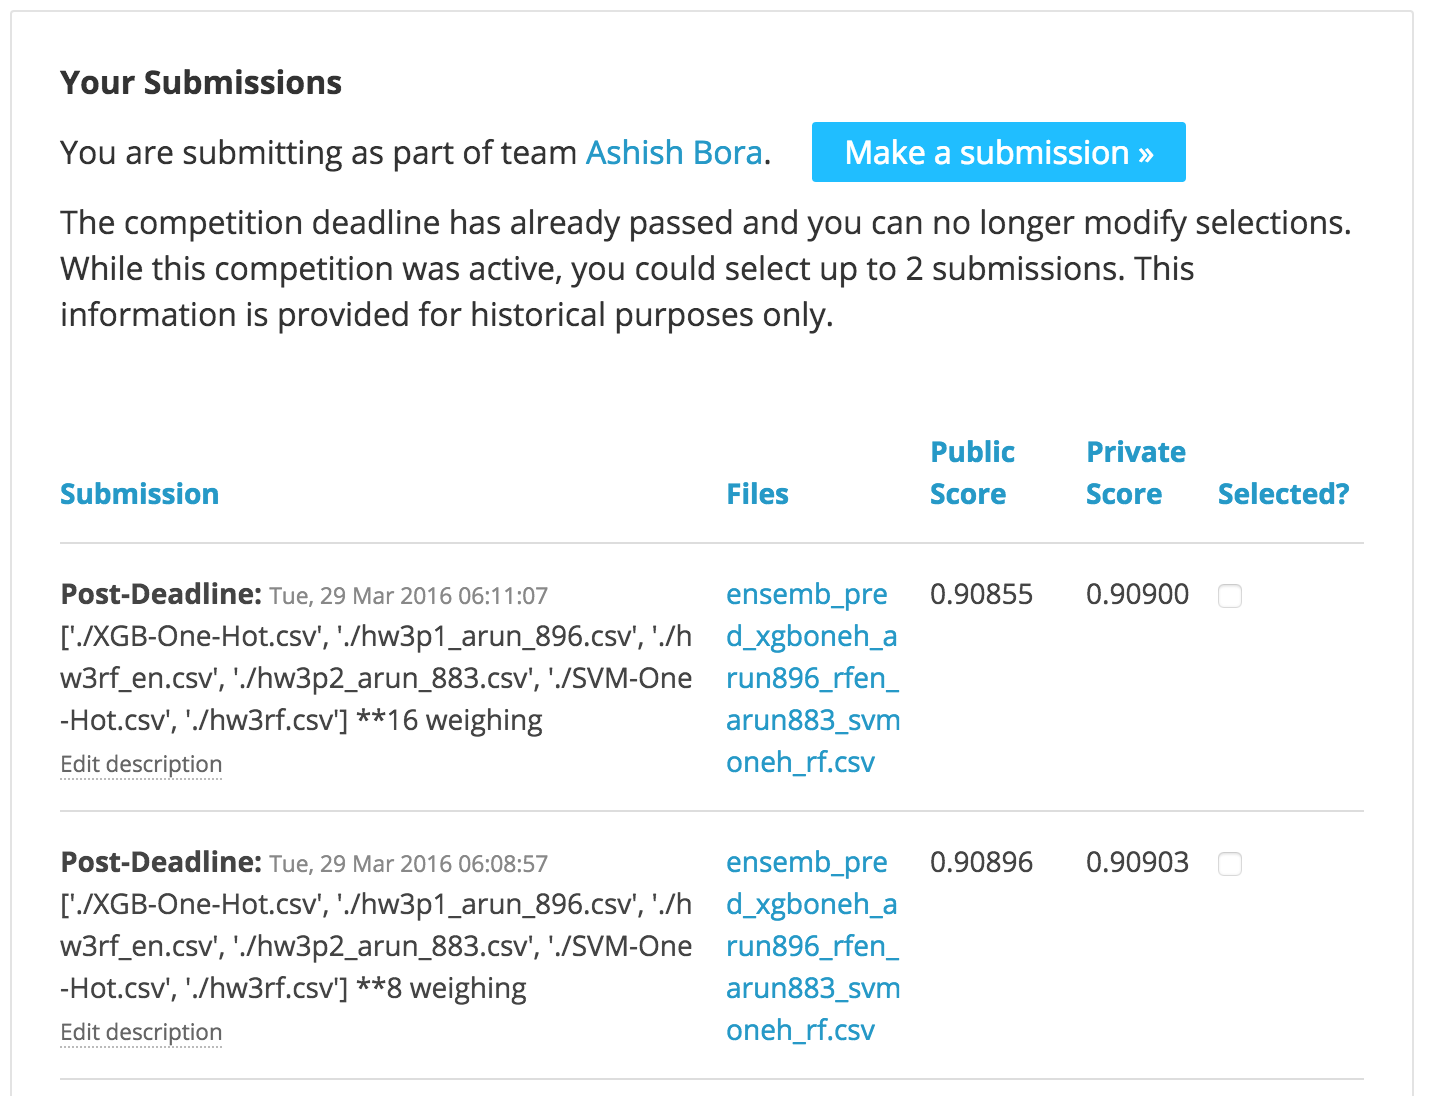
\includegraphics[width=\textwidth]{best}
\end{figure}



\end{document}
